\documentclass[11pt]{article}

\usepackage[norsk]{babel}
\usepackage[utf8]{inputenc}
\usepackage{amsmath, amssymb, amsthm, gensymb}
\usepackage{graphicx, float}
\usepackage{pstricks-add}


\author{Kjetil Kjeka}
\title{}
\date{\today}


%Slik at matriser kan defineres med linjer
\makeatletter
\renewcommand*\env@matrix[1][*\c@MaxMatrixCols c]{%
  \hskip -\arraycolsep
  \let\@ifnextchar\new@ifnextchar
  \array{#1}}
\makeatother



\begin{document}
\section{Open-loop analysis}
\subsection{Dutch-roll mode}
The complete linear model is given by $\dot{x} = A x + B u$ where \[A = \begin{bmatrix}
-0.3220 & 0.0640 & 0.0364 & -0.9917 & 0.0003 & 0.0008 \\
0 & 0 & 1 & -0.0037 & 0 & 0 \\
-30.6492 & 0 & -3.6784 & 0.6646 & -0.7333 & 0.1315 \\
8.5396 & 0& -0.0254 & -0.4764 & -0.0319 & -0.0620 \\
0 & 0 & 0 & 0 & -20.2 & 0 \\
0 & 0 & 0 & 0 & 0 & -20.2
\end{bmatrix} \]
and
\[x = \begin{bmatrix}
\beta \\
\phi \\
p \\
r \\
\delta_a \\
\delta_r 
\end{bmatrix} \]

But in the dutch roll mode only sideslip and yaw is looked upon, the model is given by $\dot{x_{dr}} = A_{dr} x_{dr} + B_{dr} \delta_r $ Where 
\[ A_{dr} = \begin{bmatrix}
-0.3220 & -0.9917 \\
8.5396 & -0.4364
\end{bmatrix} = \begin{bmatrix}
Y_v & \frac{Y_r}{V_a^* \cos{\beta^*}} \\
N_v V_a^* \cos{\beta^*} & N_r
\end{bmatrix} \]
Meaning that the charecteristic equation is given by
\[ s^2 + (-Y_v + N_r)s + (Y_v N_r - N_v Y_r) \]
Since the charecteristic equation of a general second order dynamic system is
\[s^2 + 2 \gamma \omega_0 s + \omega_0^2\]
\begin{align*}
\omega_0 &= \sqrt{Y_v N_r - N_v Y_r} &= 2.936 \\
\gamma &= \frac{1}{2} \frac{-Y_v - N_r}{\omega_0} &= 0.1292
\end{align*}
Dutch-roll mode is an aircraft motion consisting of sideslip and yaw. Depending on aircraft design this motion will be damped out to different degrees. The feeling of dutch roll has been described as ``a combination of tail-wagging and rocking from side to side''

\subsection{Spiral divergence}
The text ask to compute the spiral convergence, I'm assuming that it's the pole of the transfer function $\frac{r}{\delta_a}$, under the spiral-divergene mode assumption, that is to be computed.

It's known from Beard and McLain that: 
\[\delta_{spiral} = \frac{N_r L_v + N_v L_r}{L_v} \]
Extracting from the A matrix:
\begin{align}
&N_r &= -0.4764 \\
&\frac{N_v}{L_v} = \frac{8.5396}{-30.6492} &= -0.27862 \\
&L_r &= 0.6646
\end{align} 
Which gives
\[\delta_{spiral} = N_r - \frac{N_v}{L_v} L_r = -0.4764 - (- 0.27862) \cdot 0.6646 = -0.2912 \]



\subsection{Roll mode}
As in spiral convergence it's not completely clear what should be computed but again i assume it's the $\lambda_{rolling}$ under the assumptions of roll-mode. From the theory given in Beard and McLain this can be extracted directly from the $A$ matrix:

\[\delta_{rolling} = L_p = -3.6784\]


\section{Autopilot for course hold using succesive loop closure}
\subsection*{1}
Since this is the first time $a_{\phi 1}$ and $a_{\phi 2}$ is mentioned in this text and there is doesn't exist as much as a word what these factors are, i will assume they are as given from Figure 6.6 in Beard and McLain. In that case it's easy to see that:
\begin{align*}
& p = \frac{a_{\phi 2} }{s + a_{\phi 1} } \delta_a \\
=> & sp + a_{\phi 1} p = a_{\phi 2} \\
=> & \dot{p} = -a_{\phi 1} p + a_{phi 2} \lambda_a
\end{align*}
Then it's easy to get the coefficients from the $A$ matrix as:
\begin{align*}
a_{\phi 1} &= 3.6784 \\
a_{\phi 2} &= -0.7333
\end{align*}

\subsection*{2}
From equation (6.7), (6.8) and (6.9) in Beard and McLain, and the design parameters $\delta^{max}_a = 45 \degree$, $e^{max}_{\phi} = 15 \degree$ and $\zeta_{\phi} = 0.707$
\begin{align*}
K_{p \phi} &= \frac{\delta^{max}_a}{e^{max}_{\phi}} \hbox{sign}(a_{\phi 2}) &= -3  \\
\omega_{n \phi} &= \sqrt{\frac{\delta^{max}_a}{e^{max}_{\phi}} |a_{\phi 2}| } &= 1.4832 \\
K_{d \phi} &= \frac{2 \zeta_{\phi} \omega_{n \phi} - a_{\phi 1} }{ a_{\phi 2} } &= 2.1562
\end{align*}
Since no disturbances is modelled and there is not mentioned wich kind of disturbances that can effect the system no integrator effect will be used on the controller. If there is a constant disturbance, there should be used some kind of integral effect and/or feed forward strategy in this controller.
\[K_{i \phi} = 0\]
When designing the course controller it's important to remember that this controller is an outer loop and if it's not chosen ``slow'' enough the assumption that the pitch will follow it's reference won't hold. Beard and McLain states that adequte seperation can be achieved by chosing the design parameter $W_{\chi} > 5$, let $W_{\chi} = 10$
\[\omega_{n \chi} = \frac{1}{W_{\chi}} \omega_{n \phi} = 0.14832\]
This means that the control parameters will be:
\begin{align*}
k_{p \chi} &= 2 \zeta_{\chi} \omega_{n \chi} \frac{V_g}{g} \\
k_{i \chi} &= \omega_{n \chi}^2 \frac{V_g}{g}
\end{align*}
By trial and error $\zeta = 0.9$ seems like a good value and
\begin{align*}
k_{p \chi} &= 4.173 \\
k_{i \chi} &= 0.3438
\end{align*}
The bode plots for the transfer function $\frac{\chi}{\chi^c}$ is as shown in Figure \ref{fig:22}

\begin{figure} 
\centering
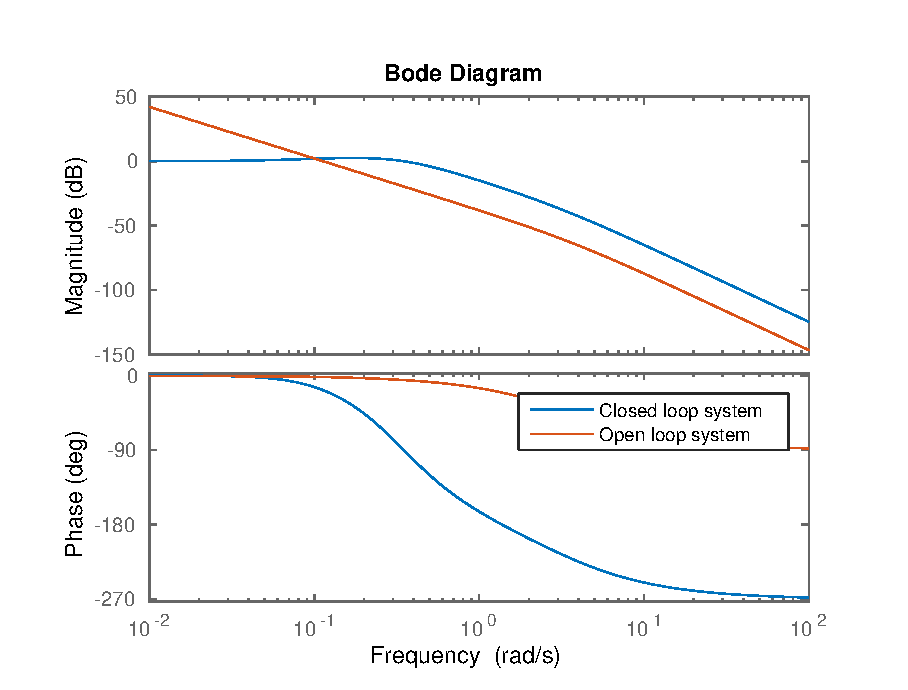
\includegraphics[width=0.9\textwidth]{fig22.eps}
\caption{Bode plots of $\frac{\chi}{\chi^c}$}
\label{fig:22}
\end{figure}


\end{document}